\documentclass[8pt]{beamer}
\usetheme{Gelugor}
\usepackage[document]{ragged2e}
\usepackage{hyperref}
\usepackage[utf8]{inputenc}
\usepackage[spanish]{babel}
\usepackage[default]{droidserif}
\usepackage{t1enc}

\title{Análisis y Diseño de Software}
\subtitle{Modelaje Colaborativo con Visual Paradigm + Github}
\author{\href{http://www.iralis.org/?q=node\%2F10&paso=10&letra=L&id=5186/}{ECINF5186} \href{http://www.iralis.org/?q=node\%2F10&paso=10&letra=L&id=5208/}{\hspace{0.5cm}ECNIF5208} \href{http://www.iralis.org/?q=node\%2F10&paso=10&letra=L&id=7223/}{\hspace{0.5cm}ECNIF7223}\\
\href{http://www.iralis.org/?q=node\%2F10&paso=10&letra=L&id=5216/}{ECNIF5216}
\href{http://www.iralis.org/?q=node\%2F10&paso=10&letra=A&id=5187/}{\hspace{0.5cm}ECINF5187}
\href{http://www.iralis.org/?q=node\%2F10&paso=10&letra=Q&id=7317/}{\hspace{0.5cm}ECINF7317}
}
\date{\today}
\institute{Ingeniería en Sistemas\\\ jalojaj@unl.edu.ec\ \hspace{0.3cm}johanna.rivera@unl.edu.ec\ \hspace{0.3cm}chjapons@unl.edu.ec\\ cepozoc@unl.edu.ec\ \hspace{0.3cm}dmarmijosa@unl.edu.ec\ \hspace{0.3cm}betty.quezada@unl.edu.ec}

\begin{document}
	
	%INICIO carátula
	\begin{frame}[plain,t]
		\titlepage
	\end{frame}
	%FIN carátula

	\section{Tema}

	\subsection{Introducción}
	\justifying
		\begin{frame}
			\frametitle{Introducción}
			%\framesubtitle{Visual Paradigm}
			\textbf{Visual Paradigm}\\
			{\small Es un herramienta poderosa, multiplataforma y fácil de utilizar para el modelado UML y herramienta CASE. Visual Paradigm proporciona a los desarrolladores de software una plataforma de desarrollo de vanguardia para construir aplicaciones de calidad más rápido, mejor y más barato!, Facilita una excelente interoperabilidad con otras herramientas CASE y la mayoría de los principales IDEs que destaca todo el proceso de desarrollo del Modelo-Code-Deploy en esta solución one-stop-shopping.} \\\
			
			\textbf{VPository}\\
			{\small VPository es el servicio en la nube que permite acceder y modificar sus diseños de software en cualquier lugar. Por otra parte, a través de diseños de software "tienda en la nube", los desarrolladores pueden conectarse a él, comprobar los proyectos que necesitan y empezar a trabajar.}
\end{frame}

\subsection{Objetivos}
\begin{frame}
\frametitle{Objetivos}
	\begin{itemize}
	\justifying
		\item Entender el funcionamiento de GitHub y VPository, mostrando las ventajas de usar cada una de estas herramientas para el trabajo de proyectos en la nube.
		\justifying
		\item Realizar un ejemplo práctico utilizando GitHub y VPository, para de esta manera llegar a tener un completo entendimiento de estas herramientas.
		\justifying
		\item Entender el funcionamiento y beneficios que nos ofrece cada una de las herramentas del repositorio Github y VPository.
	\end{itemize}
\end{frame}


\subsection{Desarrollo}
\begin{frame}
\frametitle{Desarrollo}
En el desarrollo de Aplicaciones y Sistemas, es muy importante el almacenamiento de proyectos en la nube, debido a muchos factores donde se corre el riesgo de perder parte o totalidad de éstos, por ello hoy en día existen un sinnúmero de herramientas que nos permiten almacenar proyectos y trabajar colectivamente desde cualquier parte del mundo. En este caso se hará un estudio acerca de GITHUB, y VPOSITORY, que son herramientas de alojamiento en la nube que permiten almacenar  y trabajar colectivamente con personas invitadas a colaborar en él.
\end{frame}

\subsubsection{VPository}
\begin{frame}
\frametitle{Desarrollo}

\setlength{\parskip}{15pt}
\textbf{VPository}\\
Como ya lo hemos mencionado VPository es un repositorio basado en la nube para almacenar y compartir proyectos realizados con Visual Paradigm. A los usuarios que se han suscrito a VPository se les otorga un dominio donde pueden almacenar sus proyectos. Los usuarios pueden acceder a sus cuentas VPository para comprobar los proyectos que necesitan y empezar a trabajar en ellos. Cualquier cambio que hayan hecho se pueden compartir con el resto del equipo a través de una acción de 'comit'.

\setlength{\parskip}{05pt}
\textbf{Características}\\
\begin{center}
\begin{itemize}
\item{\textbf{Colaborativo:} Permite trabajan en el mismo proyecto simultáneamente sin sobrescribir el trabajo de sus colaboradores.}
\item{\textbf{Acceso a nivel mundial:} El acceso a trabajar en diferentes proyectos es independiente de las ubicaciones geográficas de los miembros del equipo de trabajo.}
\item{\textbf{Compartir:} Los usuarios sólo necesita un navegador web para publicar y ser notificado de las actualizaciones del proyecto.}

\end{itemize}

\end{center}
\end{frame}


\begin{frame}
\frametitle{Desarrollo}

\begin{center}
\begin{itemize}
\item{\textbf{A salvo:} VPository recuerda todos los cambios realizados. Es fácil de recuperar los elementos del modelo borrado. También se realiza una copia de seguridad de todos sus proyectos diariamente para prevenir la pérdida de datos permanente.}
\item{\textbf{Seguro:} Todas las comunicaciones entre Visual Paradigm, VPository y navegador web están protegidos por la encriptación de datos SSL (misma tecnología que los bancos en línea).}
\item{\textbf{Gratis:} Permite colaborar y compartir proyectos con un almacenamiento gratuito de 1 GB. Sin obligación y sin tarjeta de crédito requerida.}

\end{itemize}

\end{center}
\end{frame}



\subsubsection{Crear una cuenta de VPository}
\begin{frame}
\frametitle{Desarrollo}

\setlength{\parskip}{10pt}
\textbf{Configuración de VPository en Visual Paradigm}\\

\setlength{\parskip}{15pt}
Para realizar la configuración del VPository en Visual Paradigm Versión Comunitaria se debe tomar en cuenta los siguientes pasos:
\begin{center}

\setlength{\parskip}{5pt}
\begin{itemize}
\item{Tener instalado Visual Paradigm Versión Comunitaria.}
\item{Abrir Visual Paradigm Versión Comunitaria.}
\item{Seleccionar la pestaña Team(Trabajo en Equipo).}
\item{Acceder a Login(Iniciar sesión).}
\item{Ok(Aceptar).}
\end{itemize} 

\setlength{\parskip}{08pt}
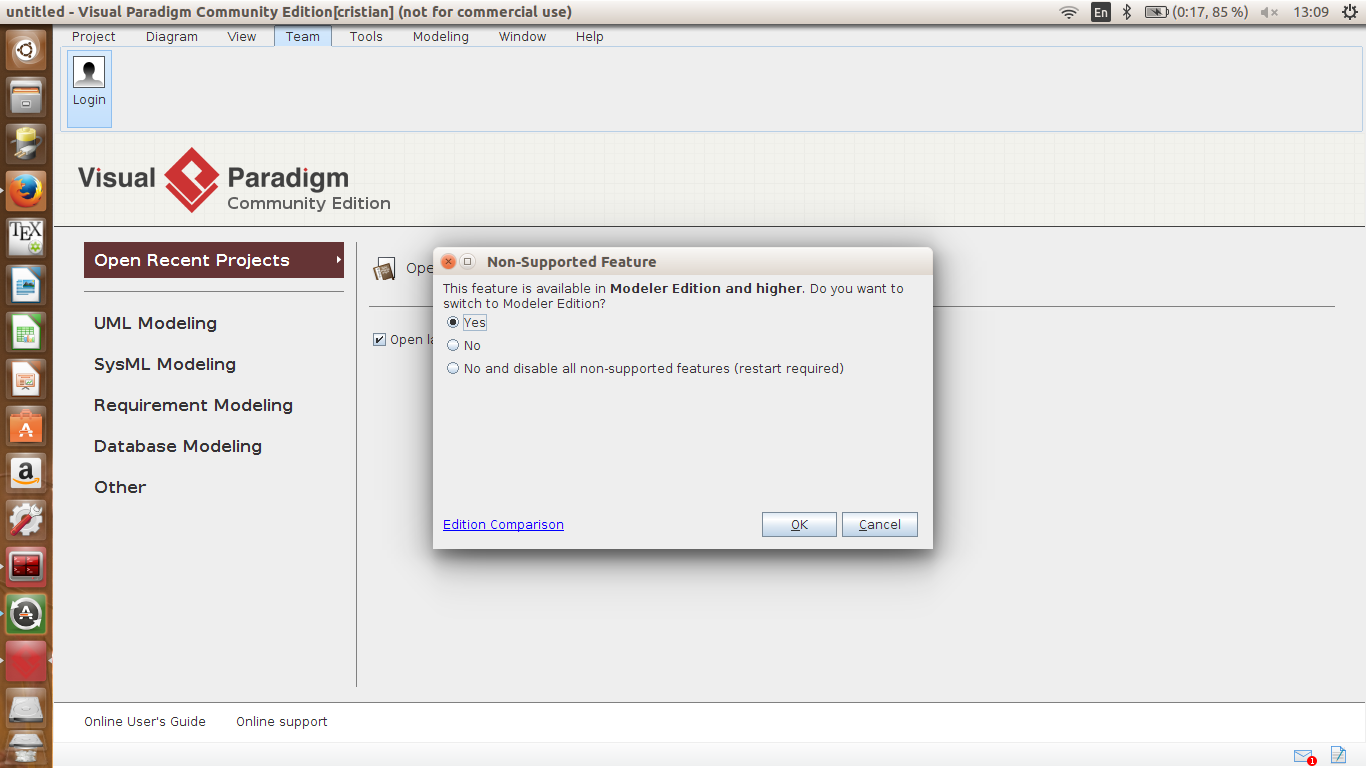
\includegraphics[width=6cm, height=3cm]{img/cap1}\\
\end{center}
\end{frame}


\begin{frame}
\frametitle{Desarrollo}

%\setlength{\parskip}{05pt}
Al abrirse la nueva ventana se procede a:

\setlength{\parskip}{03pt}
\begin{center}
\begin{itemize}
\item{Selecionar la opcion Subscribe to VPository...}
\item{Llenar todos los campos del formulario.}
\item{Seleccionar la cuadrícula aceptando los terminos y servicios de VPository.}
\item{Dar click en el botón Subscribe to VPository.}
\end{itemize} 

\setlength{\parskip}{08pt}
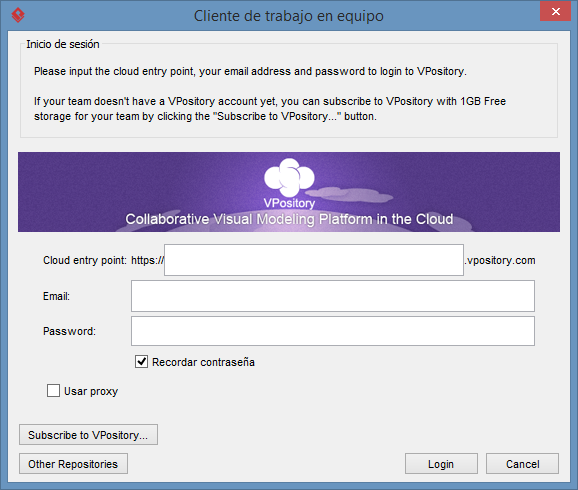
\includegraphics[width=4cm, height=3cm]{img/cap2} \hspace{0.5cm}
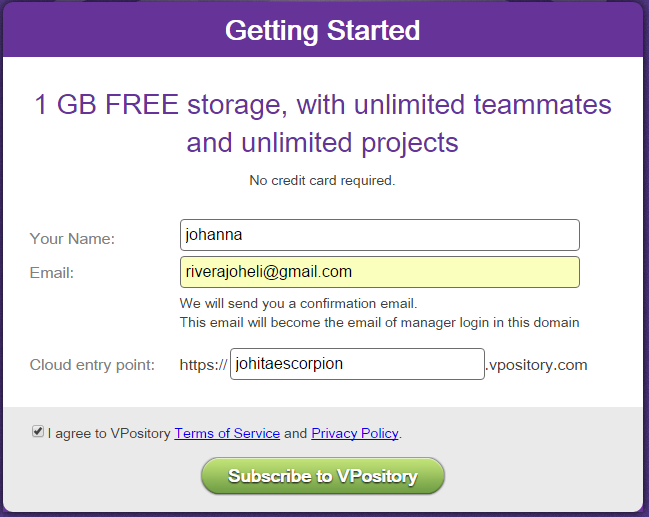
\includegraphics[width=4cm, height=3cm]{img/cap3}
%\textbf{Fig. 2 : Suscribirse a VPository }\\
\end{center}
\end{frame}


\begin{frame}
\frametitle{Desarrollo}
\setlength{\parskip}{00pt}
Al cumplir con los pasos anteriores se mostrará en pantalla una ventana notificando que se ha enviado un enlace de confirmación a la cuenta de Email proporcionada en el formulario anterior:
\begin{center}

\setlength{\parskip}{10pt}
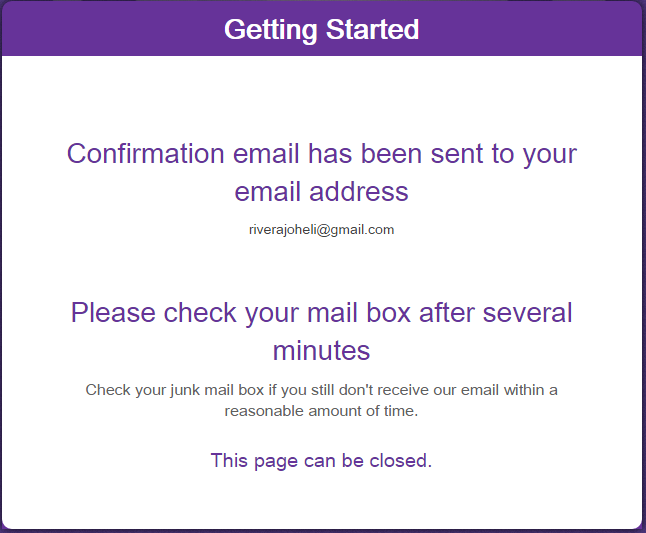
\includegraphics[width=5cm, height=3cm]{img/cap4}
%\textbf{Fig. 3 : Confirmación VPository }
\end{center}
\end{frame}


\begin{frame}
\frametitle{Desarrollo}
\setlength{\parskip}{05pt}
Para finalizar con la subscripción es necesario abrir nuestro correo y dirigirnos al mensaje recibido de VPository.
\begin{itemize}
\item{Abrir el mensaje recibido de VPository.}
\item{Click en el enlace Confirm your VPository Subscription.}
\item{Llenar todos los campos del formulario para iniciar sesion con nuestra nueva cuenta de VPository.}
\item{Click en el botón Start My VPository.}
\end{itemize} 
\begin{center}
\setlength{\parskip}{08pt}
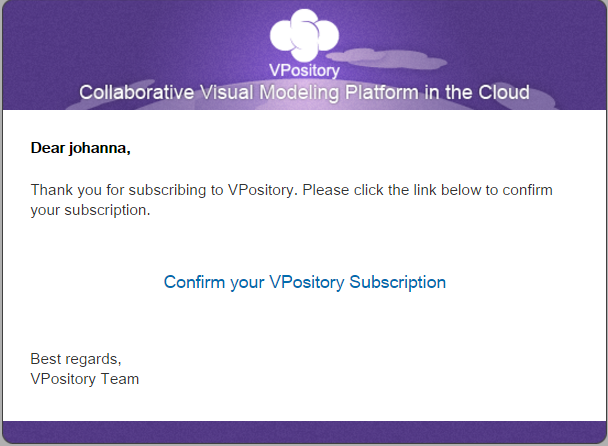
\includegraphics[width=4cm, height=3cm]{img/cap5}\hspace{0.5cm}
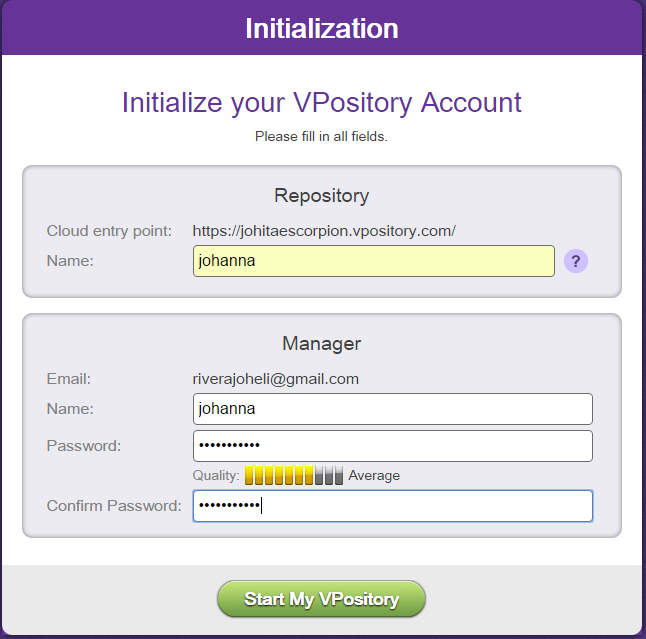
\includegraphics[width=4cm, height=3cm]{img/cap6}
\end{center}
\end{frame}


\begin{frame}
\frametitle{Desarrollo}
\setlength{\parskip}{05pt}
Al terminar correctamente la subscripción nos mostrará en pantalla un mensaje de éxito.
\begin{center}

\setlength{\parskip}{08pt}
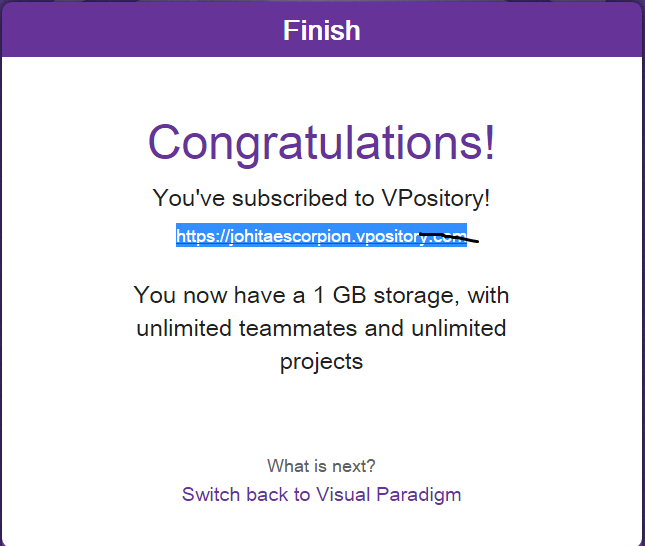
\includegraphics[width=6cm, height=3cm]{img/cap7}\\
\end{center}
\end{frame}


\subsubsection{Creación de un proyecto colaborativo VPository}
\begin{frame}
\frametitle{Desarrollo}

\setlength{\parskip}{05pt}
Terminada la creación de nuestra cuenta VPository, podemos ya iniciar sesión con Visual Paradigm.
\begin{center}

\setlength{\parskip}{06pt}
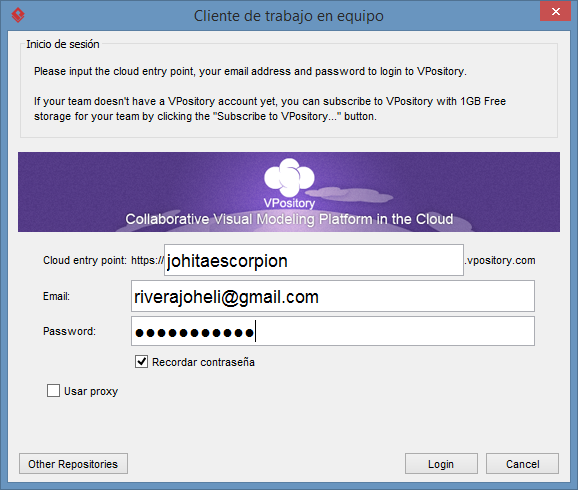
\includegraphics[width=5cm, height=3cm]{img/cap8}
\end{center}

Ya que aun no tenemos proyetos en nuestra cuenta se mostrará un mensaje para importar o crear un  nuevo proyecto.
\begin{center}
\setlength{\parskip}{08pt}
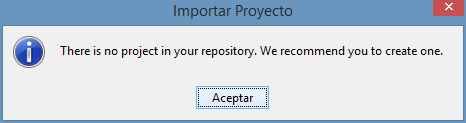
\includegraphics[width=5cm, height=1cm]{img/cap9}
\end{center}
\end{frame}


\begin{frame}
\frametitle{Desarrollo}
Al abrirse la nueva ventana se procede a:

\setlength{\parskip}{03pt}
\begin{center}
\begin{itemize}
\item{Colocar un nombre al nuevo proyecto}
\item{El autor del proyecto.}
\item{Typo de proyecto.}
\item{colocar una descripción del nuevo proyecto.}
\item{Selecionamos el botón Add Proyect Member para agregar más colaboradores.}
\end{itemize} 

\setlength{\parskip}{08pt}
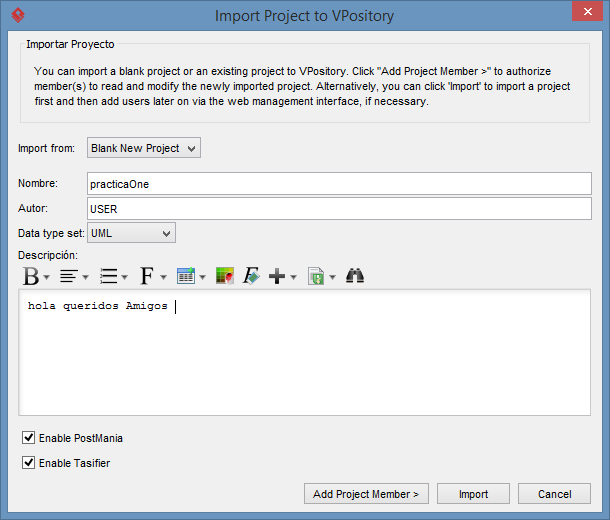
\includegraphics[width=4cm, height=3cm]{img/cap10} \hspace{0.5cm}
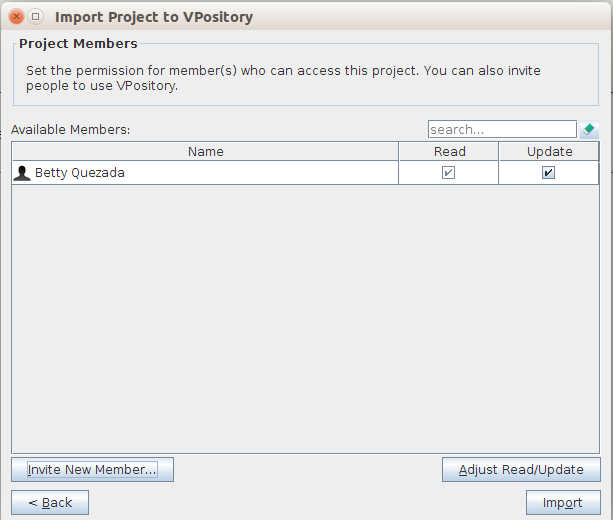
\includegraphics[width=4cm, height=3cm]{img/cap11}
%\textbf{Fig. 2 : Suscribirse a VPository }\\
\end{center}
\end{frame}


\begin{frame}
\frametitle{Desarrollo}
Procedemos agregar todos los colaboradores necesarios:

\setlength{\parskip}{03pt}
\begin{center}
\begin{itemize}
\item{Click en Invite New Member...}
\item{Ingresar el nombre de usuarios como estén registrados.}
\item{Ingresar su Email.}
\item{Seleccionar el boton Ok.}
\item{Seleccionar el boton Import.}
\end{itemize} 

\setlength{\parskip}{08pt}
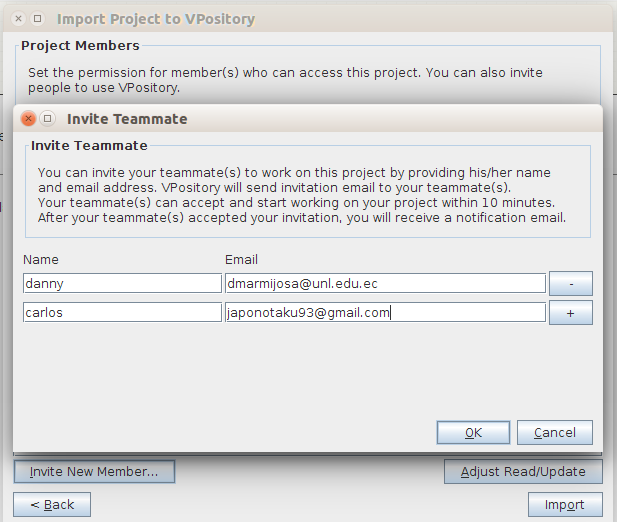
\includegraphics[width=4.5cm, height=3cm]{img/cap12} \hspace{0.5cm}
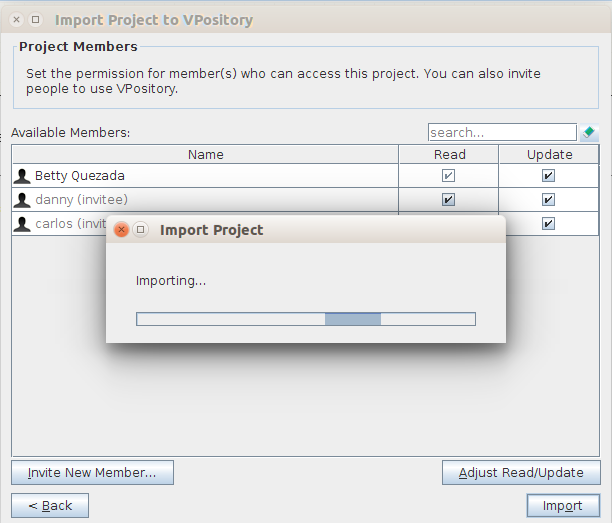
\includegraphics[width=4.5cm, height=3cm]{img/cap13}
\end{center}
\end{frame}


\begin{frame}
\frametitle{Desarrollo}
Al momento de ser agregado como colaborador de un nuevo proyecto, es necesario validar la colaboración mediante el enlace enviado a nuestro Email.

\setlength{\parskip}{03pt}
\begin{center}
\begin{itemize}
\item{Abrir el mensaje recibido en nuestro Email.}
\item{Selecionar el enlace Active your VPository account.}
\end{itemize} 

\setlength{\parskip}{08pt}
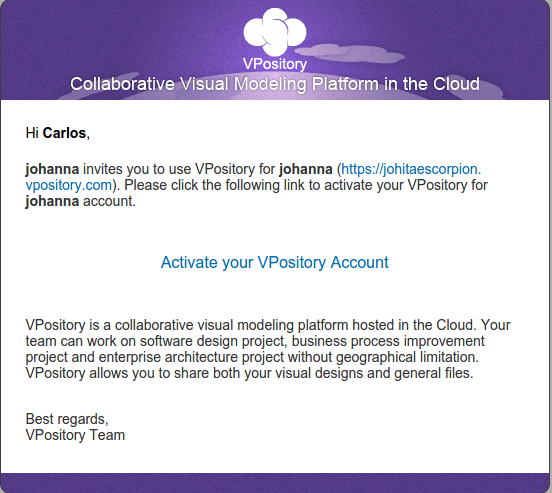
\includegraphics[width=06cm, height=4cm]{img/cap16}
%\textbf{Fig. 2 : Suscribirse a VPository }\\
\end{center}
\end{frame}


\begin{frame}
\frametitle{Desarrollo}
Procedemos a llenar los campos del formulario con nuestros datos, sin importar que la cuenta sea de quien nos haya echo la invitación.

\setlength{\parskip}{03pt}
\begin{center}
\begin{itemize}
\item{Ingresar su Email.}
\item{Ingresar su contraseña.}
\item{Click en el botón Login}
\item{Click en el icono Tasifier para ver el proyecto a colaborar}
\end{itemize} 

\setlength{\parskip}{08pt}
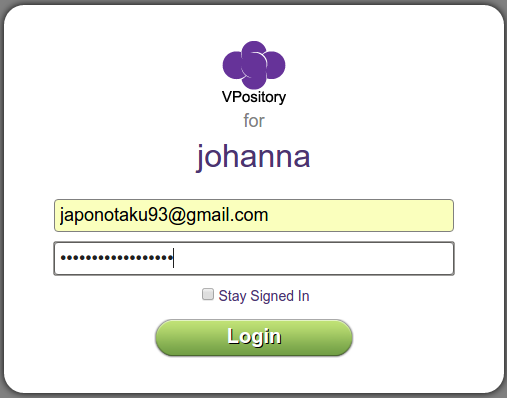
\includegraphics[width=4.5cm, height=3cm]{img/cap17} \hspace{0.5cm}
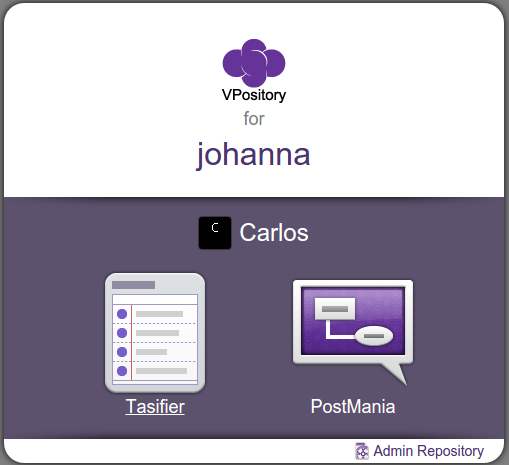
\includegraphics[width=4.5cm, height=3cm]{img/cap18}
%\textbf{Fig. 2 : Suscribirse a VPository }\\
\end{center}
\end{frame}


\begin{frame}
\frametitle{Desarrollo}
\setlength{\parskip}{10pt}
Al verificar el proyecto a colaborar ya podemos iniciar a trabajar en él mismo, para esto deberemos cerrar la cerrar sesión actual en visual paradigm. Team->Utilities->Logout.

\setlength{\parskip}{02pt}
\begin{center}
\begin{itemize}
\item{Selecionamos Team->Login.}
\item{Click en el botón Other Repositories.}
\item{Llenar el campo URL con la dirección donde se va a colaborar.}
\item{Ingresar nuestro Email y contraseña}
\item{Seleccionar la cuadricula (We host Teamwork Server in our own web server).}
\item{Click en el botón Login.}
\end{itemize} 

\setlength{\parskip}{08pt}
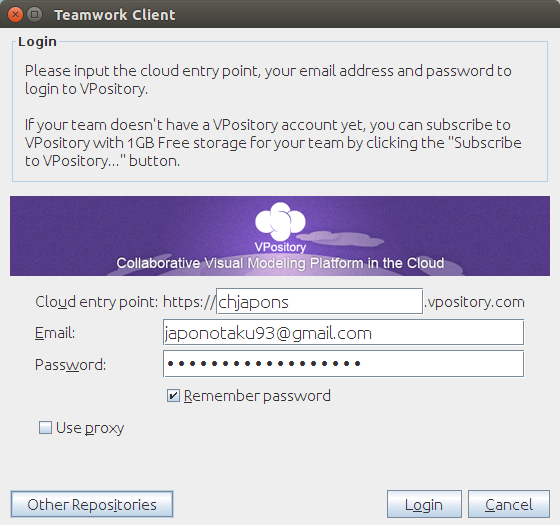
\includegraphics[width=4.5cm, height=3cm]{img/cap19} \hspace{0.5cm}
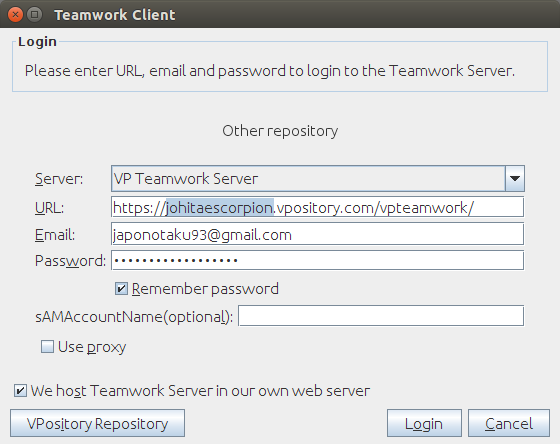
\includegraphics[width=4.5cm, height=3cm]{img/cap20}
%\textbf{Fig. 2 : Suscribirse a VPository }\\
\end{center}
\end{frame}

\begin{frame}
\frametitle{Desarrollo}
\setlength{\parskip}{10pt}
Al lograr iniciar sesión correctamente se visualizará el proyecto a trabajar.

\setlength{\parskip}{02pt}
\begin{center}
\setlength{\parskip}{08pt}
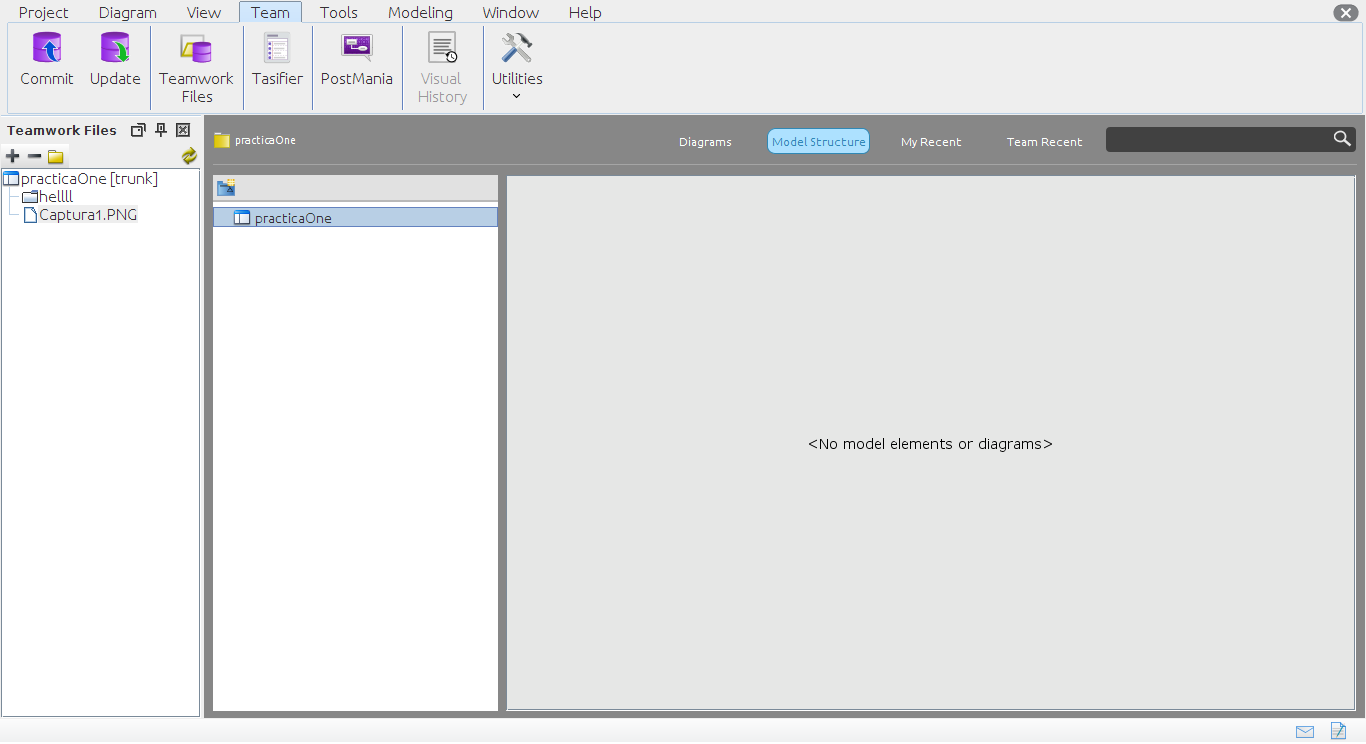
\includegraphics[width=6cm, height=4cm]{img/cap22} 
%\textbf{Fig. 2 : Suscribirse a VPository }\\
\end{center}
Como nota adicional cada vez que se desee guardar los cambios realizados en el proyecto actual, es necesario seleccionar el ícono Commit, para registrar y notificar a los demas colaboradores del proyecto.
\end{frame}

\begin{frame}
\frametitle{Desarrollo}
\setlength{\parskip}{10pt}
Se podrá trabajar con varios proyectos del mismo anfitrion, ya que si se desea trabajar con proyectos de otros usuarios, será necesario cerrar la sesión y abrir nuevamente con la dirección de dominio del anfitrion del proyecto a trabajar.

\setlength{\parskip}{02pt}
\begin{center}
\setlength{\parskip}{08pt}
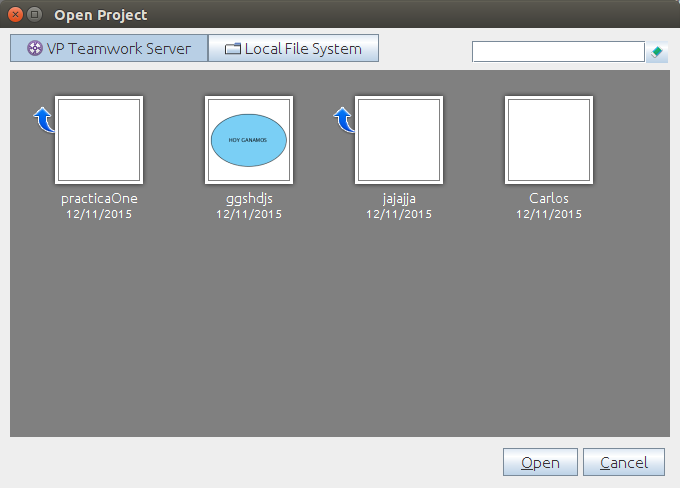
\includegraphics[width=6cm, height=3cm]{img/cap21} 
%\textbf{Fig. 2 : Suscribirse a VPository }\\
\end{center}
\end{frame}


\begin{frame}
\frametitle{Desarrollo}
El trabajo en Equipo(Team) de visual Paradigm, nos ofrece una herramienta esencial para el trabajo con VPository.\\\

\textbf{¿PostMania?}\\

PostMania es una herramienta incluida con VPository que permite compartir los diagramas creados en Visual Paradigm con otros, y para recoger sus comentarios. Muy a menudo, se comparte diagramas con socios, clientes o colegas para hacerles confirman o aclaran cuestiones de diseño. Para esto existen dos maneras.

\begin{itemize}
\justifying
\item{\textbf{A través de una invitación.} }\\

Para esto es necesario conocer el nombre y/o la dirección de correo electrónico de las personas a compartir. PostMania enviará correos electrónicos de invitación a todas las personas indicadas.\\

%\setlength{\parskip}{2mm}
\justifying
\item{ \textbf{A través de un enlace compartido.} }\\

Se puede dar una URL para abrir el diagrama en un navegador web, una vez conectado se puede ver el diagrama compartido.
\end{itemize}
\end{frame}








%///////////////////////////////////////////////////////////////////////////////////////
\subsubsection{GITHUB}
\begin{frame}
\frametitle{GITHUB}
\textbf{¿Qué es GitHub?}\\

GitHub es una plataforma de desarrollo colaborativo de software para alojar proyectos en la nube utilizando el sistema de control de versiones Git.\\\

\textbf{¿Para que sirve?}\\

GitHub aloja proyectos y brinda herramientas muy útiles para el trabajo en equipo. Para poder alcanzar esta meta, GitHub provee de funcionalidades para hacer un fork y solicitar pulls. Una vez realizadas tus modificaciones puedes enviar un pull al dueño del proyecto. Éste podrá analizar los cambios que has realizado fácilmente, y si considera interesante tu contribución, adjuntarlo con el repositorio original.
\end{frame}

\begin{frame}
\frametitle{Acerca de Git Hub}
\textbf{¿Qué herramientas proporciona?}\\
\begin{itemize}
\item Una wiki para el mantenimiento de las distintas versiones de las páginas.
\item Un sistema de seguimiento de problemas que permiten a los miembros de tu equipo detallar un problema con tu software o una sugerencia que deseen hacer.
\item Una herramienta de revisión de código.
\item Un visor de ramas donde se pueden comparar los progresos realizados en las distintas ramas de nuestro repositorio.
\end{itemize}
\end{frame}


\begin{frame}
\frametitle{Acerca de Git Hub}
Para utilizar esta herramienta hemos considerdado poner ciertos conceptos de la herramienta GITHUB.
\begin{itemize}
\justifying
\item {Todo acceso a la API es a través de HTTPS, y se accede desde el \url{api.github.com}, todos los datos se envían y se reciben como JSON(JavaScript Object Notation).Campos en blanco se incluyen como null en lugar de ser omitido.}
\justifying
\item {Todas las marcas de tiempo se devuelven en formato ISO 8601}
\justifying
\item {Todos los objetos de error tienen propiedades de los recursos y sobre el terreno para que su cliente puede decir cuál es el problema. También hay un código de error para hacerle saber lo que está mal con el campo.}
\justifying
\item {Para las solicitudes que utilizan la autenticación básica o OAuth, puede realizar hasta 5.000 solicitudes por hora. Para las solicitudes no autenticadas, el límite de velocidad le permite hacer hasta 60 solicitudes por hora. Las solicitudes no autenticadas están asociados con su dirección IP, y no el usuario que realiza peticiones.}
\end{itemize}
\end{frame}


\begin{frame}
\frametitle{Acerca de Git Hub}
\begin{itemize}
\justifying
\item {Cuenta Servicios de cortafuegos y VPN dedicados para ayudar a bloquear el acceso no autorizado al sistema.}
\justifying
\item{compensación por medio de un pago realizado en paypal para las personas que cazan vulnerabilidades en el sistema, y debe aculumar cierta cantidad de puntos. Un ejemplo de vurnerabilidades y sus respectivos  cazadores estan publicadas en \url{https://bounty.github.com/}  }
\justifying
\item {Para  evolucionar emmpresarialmente GIT HUB contrata desarrolladores, los cuales deben estar registrados y tener un plan de pagos. Si cumple con esos requisitos pueden entrar a url{https://developer.github.com/program/}}
\justifying
\item {Git Hub utiliza el codigo de las cuentas  gratuitas para mejorar su plataforma virtual.}
\justifying
\item{compensación por medio de un pago realizado en paypal para las personas que cazan vulnerabilidades en el sistema, y debe aculumar cierta cantidad de puntos. Un ejemplo de vurnerabilidades y sus respectivos  cazadores estan publicadas en \url{https://bounty.github.com/}  }
\end{itemize}
\end{frame}

\begin{frame}
\frametitle{Acerca de Git Hub}
\begin{itemize}

\justifying
\item {Para  evolucionar emmpresarialmente GIT HUB contrata desarrolladores, los cuales deben estar registrados y tener un plan de pagos. Si cumple con esos requisitos pueden entrar a \url{https://developer.github.com/program/}.}
\justifying
\item {Git Hub utiliza el codigo de las cuentas  gratuitas para mejorar su plataforma virtual.}
\justifying
\item{Git: Es un software de control de versiones diseñado por Linus Torvalds, pensando en la eficiencia y la confiabilidad del mantenimiento de versiones de aplicaciones cuando estas tienen un gran número de archivos de código fuente.}
\justifying  
\item{Git Hub: Es una forja para alojar proyectos utilizando el sistema de control de versiones Git. Utiliza el framework Ruby on Railspor GitHub, Inc. }
\justifying
\item {Git Hub forma parte de git, lo cual git instalado en nuestro sistema operativo \textbf{Linux,Mac,Windows y Solaris} nos permite subir nuestro archivos a nuestro repositorio Git-Hub, utilizando los comandos de git en su respectivo Sistema Operativo. }
\end{itemize}
\end{frame}

\begin{frame}
\frametitle{Git y Git Hub}
\begin{itemize}
\justifying
\item{Git tiene una api de comandos (\url{https://git-scm.com/docs/}) que se puede utilizar en nuestro sistema Operativo de preferencia ya sea linux, windows y mac.}
\justifying
\item{Para aprendizaje de los comandos de git en nuestros  sistemas operativos, git tiene una plataforma la cual es \url{https://try.github.io},en donde el objetivo de esta herramienta es que no sea un obstaculo el manejo de git en nuestros SO.}


\end{itemize}
\end{frame}





\subsubsection{Instalación y configutación de GITHUB}

%/////////////////////////////////////////

%/////////////////////////////////////////////

\begin{frame}
\frametitle{Desarrollo}

\setlength{\parskip}{10pt}
\textbf{Vinculación de Git-Hub con el Sistema Operativo Ubuntu.}\\

\setlength{\parskip}{15pt}
Para realizar la vinculación del Git - Hub en el sistema operativo Ubuntu se debe realizar los siguientes pasos:
\begin{center}

\setlength{\parskip}{5pt}
\begin{itemize}
\item{Tener una cuenta creada en la pagina \url{www.github.com}.}
\item{Tener lista la carpeta  para la  vinculación con el GitHub. }
\end{itemize} 

\setlength{\parskip}{08pt}
\end{center}
\end{frame}



%Creación de la Cuenta Git Hub
\begin{frame}
\frametitle{Desarrollo}

%\textbf{Creación de la Cuenta Git Hubs}

%\setlength{\parskip}{05pt}
Para lograr vincular nuestro sistema operativo con github.com necesitamos crear una cuenta en \url{www.github.com}. 
\setlength{\parskip}{03pt}
\begin{center}
\begin{itemize}
\item{Abrimos el navegador web de preferencia y colocamos la url \url{www.github.com/join}.}
\item{Llenar todos los campos del formulario.}
\item{Dar click en Create an account}
\item{Seleccionar el plan de pago y dar click en Finish sign up}
\end{itemize} 

\setlength{\parskip}{08pt}
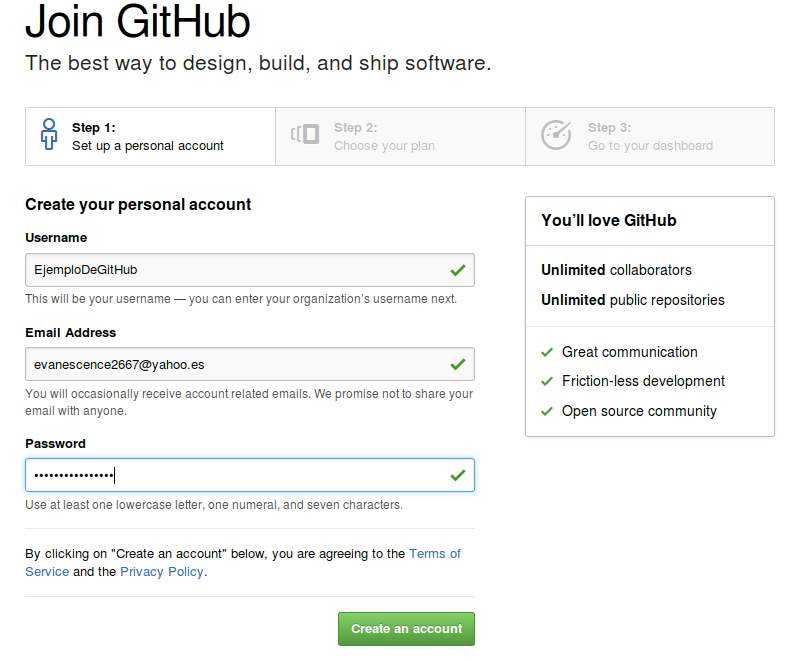
\includegraphics[width=4cm, height=3cm]{img/uno} \hspace{0.5cm}
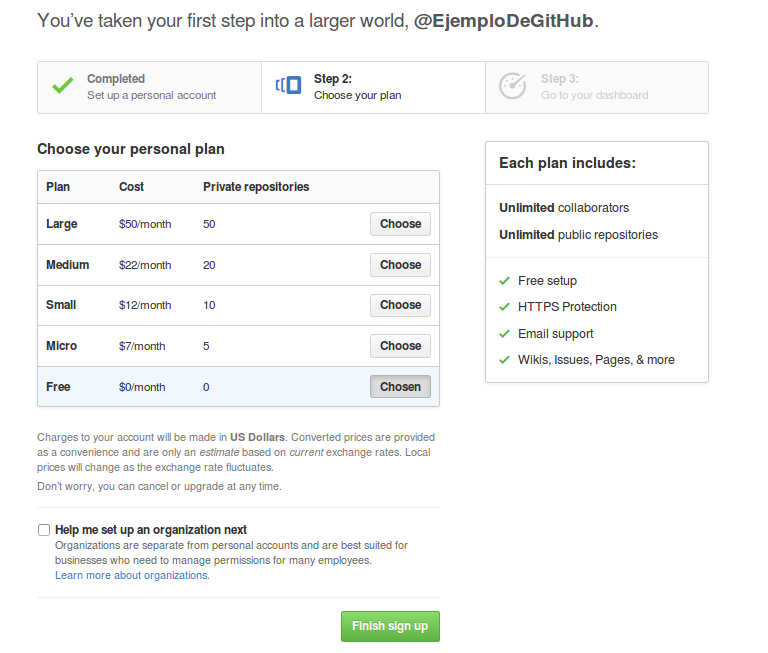
\includegraphics[width=4cm, height=3cm]{img/dos}
%\textbf{Fig. 2 : Suscribirse a VPository }\\
\end{center}
\end{frame}





\begin{frame}
\frametitle{Desarrollo}

%\textbf{Creación del repositorio en Git Hub}

%\setlength{\parskip}{05pt}
Para lograr vincular nuestro sistema operativo con \url{www.github.com} necesitamos primeramente crear nuestro repositorio en la nube. 

\setlength{\parskip}{03pt}
\begin{center}
\begin{itemize}
\item{Abrimos un navegador web, luego entramos a la siguiente url \url{www.github.com/login}y llenamos los datos con la cuenta que hayamos creado}
\item{Llenar los campos del formulario.}
\item{Seleccionar la el checkbox Initialize this repository with a README, }
\item{Dar click en el botón Create repository.}
\end{itemize} 



\setlength{\parskip}{08pt}
%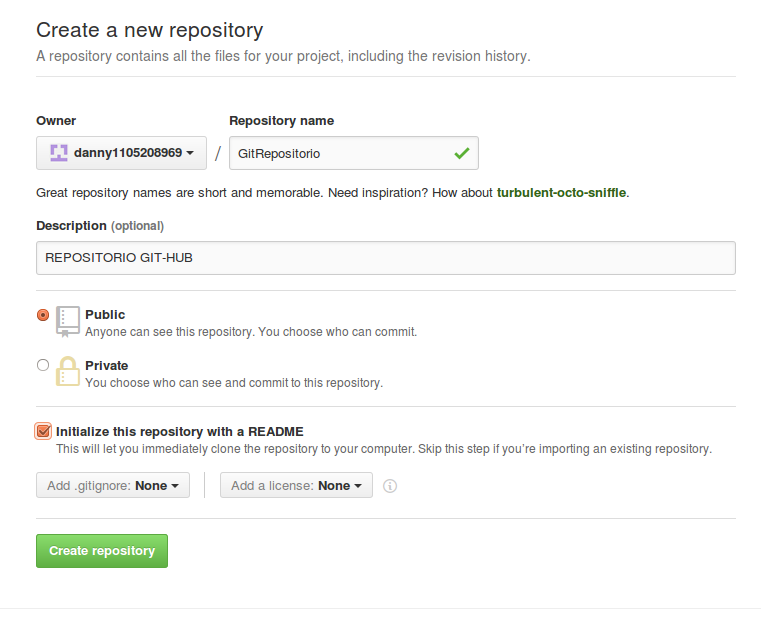
\includegraphics[width=5cm, height=3cm]{img/tres} \hspace{0.5cm}
%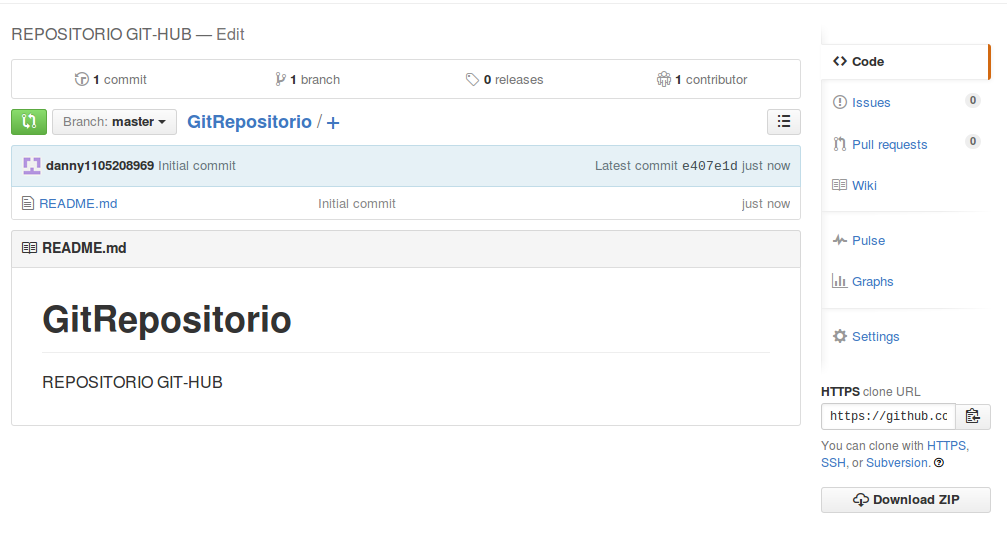
\includegraphics[width=4cm, height=3cm]{img/cuatro}
%\textbf{Fig. 2 : Suscribirse a VPository }\\
\end{center}
\end{frame}


\begin{frame}
\frametitle{Desarrollo}

%\textbf{Instalación del Git Core y Creación de la carpeta para el repositorio}

%\setlength{\parskip}{05pt}
Para subir los datos a nuestro repositorio Git Hub, tendremos que instalar la herramienta de Git Hub para linux, y crear una carpeta del repositorio donde haremos la vinculación con nuestro repositorio en la nube. 

\setlength{\parskip}{03pt}
\begin{center}
\begin{itemize}
\justifying
\item{Abrimos una terminal ya sea con el Dashboard o con las combinacion del teclado CTRL+ALT+T}
\item{Colocamos el comando \textbf{sudo apt-get install git-core} despues nos pedira la contraseña que tengamos el linux, la cual la escribiremos y luego presionamos la tecla ENTER.}
\justifying
\item{Una vez Instalado en nuestro Equipo, aprovecharemos que el terminal de linux abierto para la creación de la carpeta con cualquier nombre, para ello escribiremos el comando  \textbf{mkdir NombreDeLaCarpeta}  y presionamos la tecla ENTER}
\end{itemize} 

\setlength{\parskip}{08pt}
%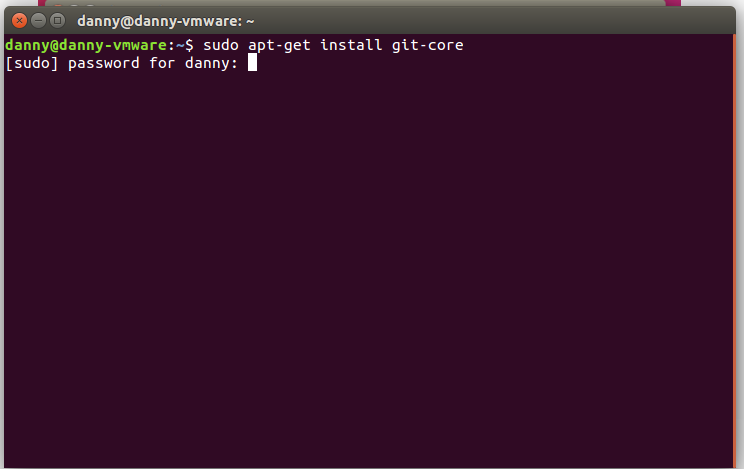
\includegraphics[width=4.5cm, height=3cm]{img/cinco} \hspace{0.5cm}
%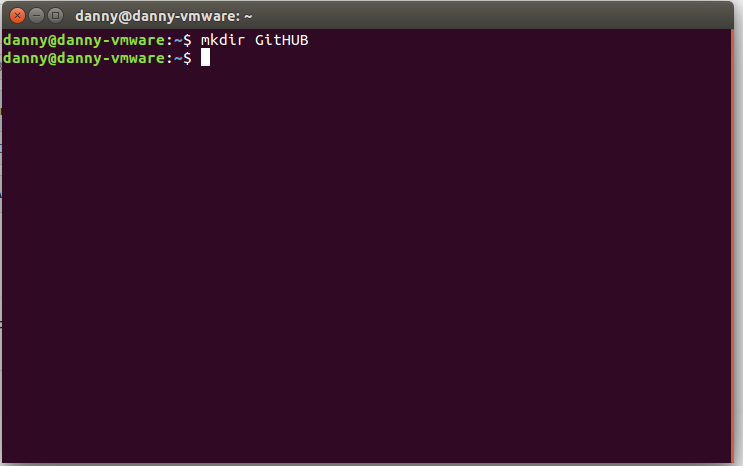
\includegraphics[width=4.5cm, height=3cm]{img/seis}
%\textbf{Fig. 2 : Suscribirse a VPository }\\
\end{center}
\end{frame}



\begin{frame}
\frametitle{Desarrollo}

%\textbf{Agregar el repositorio a la carpeta de nuestras computadoras}

%\setlength{\parskip}{05pt}
Para agregar el repositorio que hemos creado en \url{www.github.com}, ingresaremos a la carpeta desde el terminal y tambien ingresaremos a la a nuestro repositorio para obtener la url del mismo. 

\setlength{\parskip}{03pt}
\begin{center}
\begin{itemize}
\justifying
\item{Para ingresar a la carpeta que hemos creado lo haremos mediante el comando \textbf{cd NombreDeLaCarpeta}}
\justifying
\item{Para obtener la dirección url del repositorio abrimos el navegador de preferencia, nos dirigimos al repositorio que hemos creado y en una parte derecha de la pagina web estara la url que necesitamos.}
\end{itemize} 

\setlength{\parskip}{03pt}
%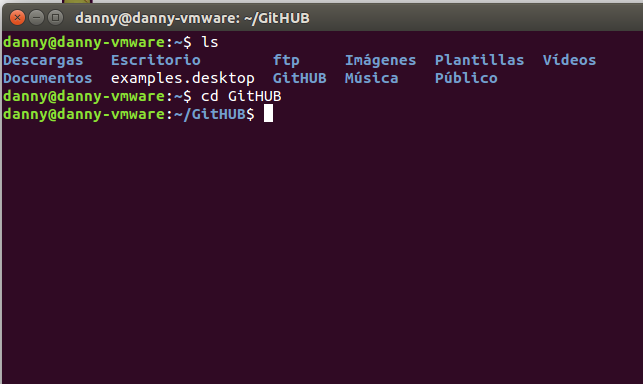
\includegraphics[width=5cm, height=3cm]{img/siete} \hspace{0.5cm}
%\textbf{Fig. 2 : Suscribirse a VPository }\\
\end{center}
\end{frame}

\begin{frame}
\setlength{\parskip}{10pt}
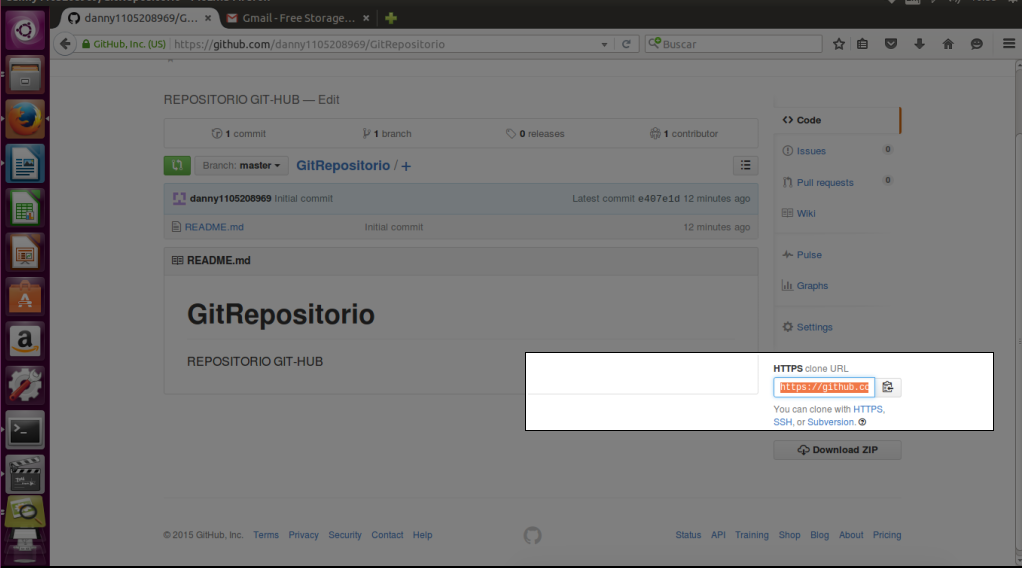
\includegraphics[width=10cm, height=7cm]{img/ocho}
\end{frame}

\begin{frame}
\frametitle{Desarrollo}
\setlength{\parskip}{00pt}
Para finalizar con la clonacion del repositorio en la nube tendremos que colocar el siguiente codigo en el terminal \textbf{git clone UrlObtenidaDelRepositorio} y luego comprobar que si se ha clonado con exito abriendo la carpeta que hemos creado y observar si nuestro repositorio esta con su archivo README. 
\begin{center}

\setlength{\parskip}{08pt}
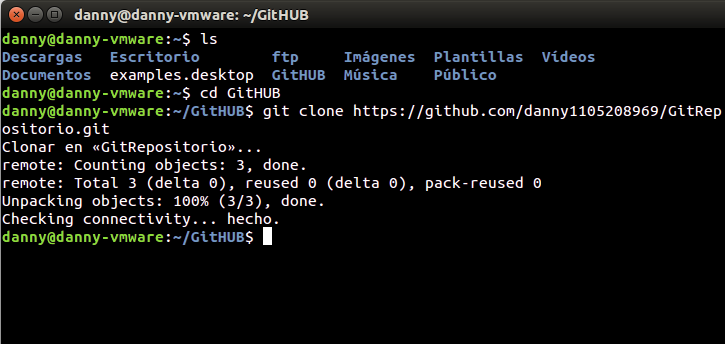
\includegraphics[width=5cm, height=3cm]{img/nueve} \hspace{0.5cm}
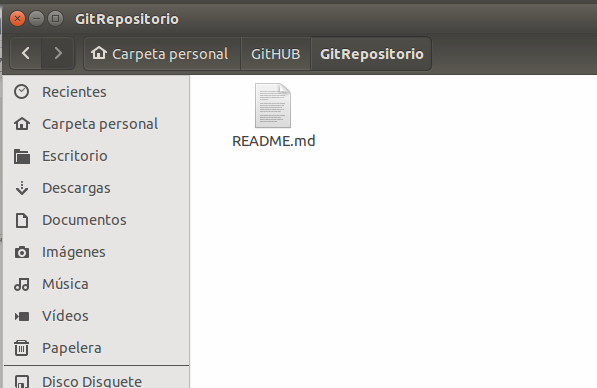
\includegraphics[width=4cm, height=3cm]{img/diez}
%\textbf{Fig. 3 : Confirmación VPository }
\end{center}
\end{frame}


\begin{frame}
\frametitle{Desarrollo}

\textbf{Subir un Proyecto de Visual Paradigm al repositorio.}

%\setlength{\parskip}{05pt}
Para subir los datos a nuestro repositorio Git Hub, tendremos que instalar la herramienta de Git Hub para linux Git Gui, colocar todo la carpeta del proyecto de Visual Paradigm a la carpeta que clonamos anteriormente y dar los respectivos permisos. 

\setlength{\parskip}{03pt}
\begin{center}
\begin{itemize}
\justifying
\item{Colocamos el comando \textbf{sudo apt-get install gitk giggle git-cola git-gui gitg} despues nos pedira la contraseña que tengamos el linux, la cual la escribiremos y luego presionamos la tecla ENTER.}
\end{itemize} 

\setlength{\parskip}{01pt}
%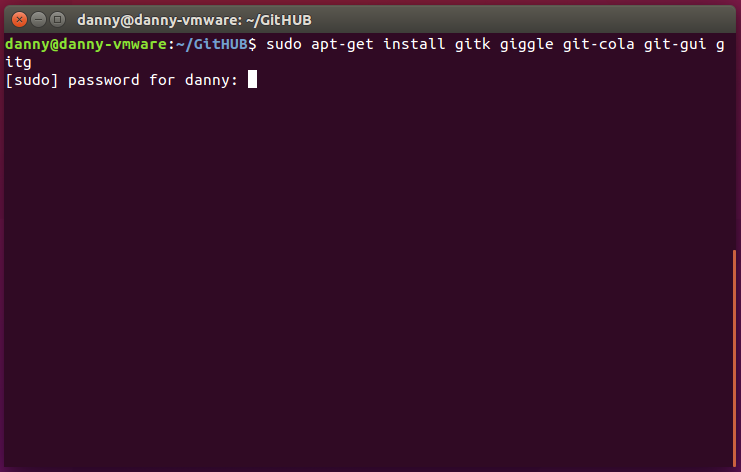
\includegraphics[width=4.5cm, height=3cm]{img/once} 
%\textbf{Fig. 2 : Suscribirse a VPository }\\
\end{center}
\end{frame}


\begin{frame}
\frametitle{Desarrollo}

\setlength{\parskip}{03pt}
\begin{center}
\begin{itemize}
\justifying
\item{Una vez Instalado en nuestro Equipo, aprovecharemos que el terminal de linux abierto y colocaremos el siguiente comando \textbf{git gui} y seleccionamos la tercera opción y buscamos el .gib para la vinculación de la carpeta de ubuntu al repositorio .}\end{itemize} 

\setlength{\parskip}{08pt}
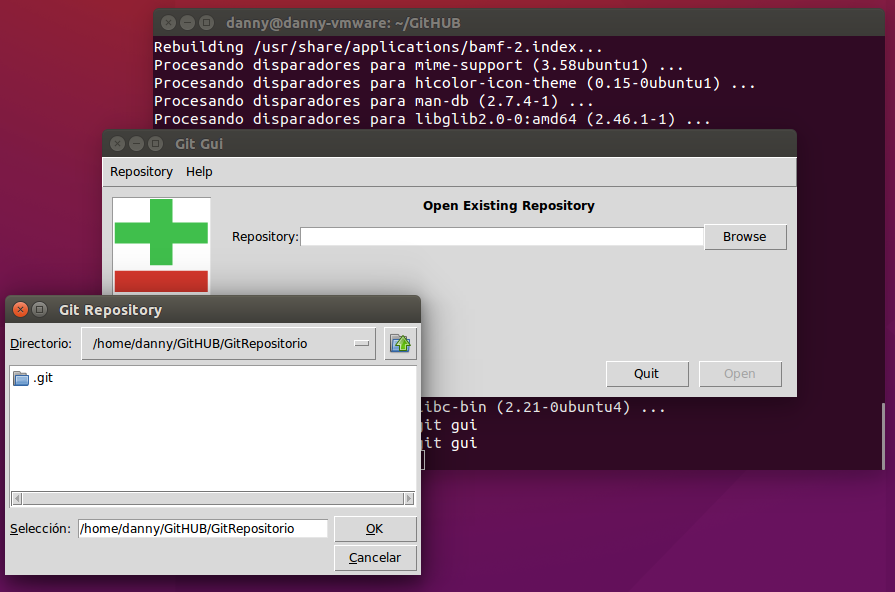
\includegraphics[width=8cm, height=5cm]{img/doce}
%\textbf{Fig. 2 : Suscribirse a VPository }\\
\end{center}
\end{frame}



\begin{frame}
\frametitle{Desarrollo}

\setlength{\parskip}{03pt}
\begin{center}
\begin{itemize}
\justifying
\item{ Despues saldra una ventana de error la cual solo sale si el lenguaje del sistema operativo no es ingles, en el caso que el lenguaje no sea ingles solo se hace un clic en el boton ok.}\end{itemize} 

\setlength{\parskip}{08pt}
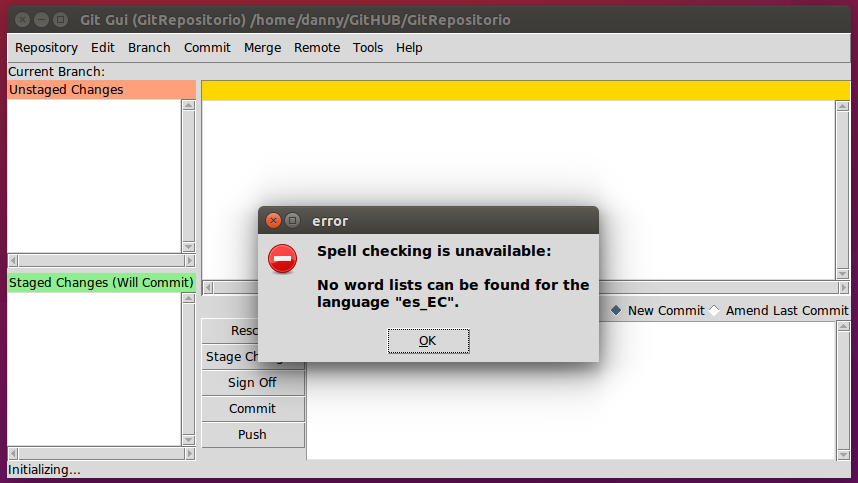
\includegraphics[width=8cm, height=5cm]{img/trece}
%\textbf{Fig. 2 : Suscribirse a VPository }\\
\end{center}
\end{frame}



\begin{frame}
\frametitle{Desarrollo}

\setlength{\parskip}{03pt}
\begin{center}
\begin{itemize}
\justifying
\item{Cerraremos la ventana de git gui y luego colocaremos el proyecto que queramos subir al github en nuestra carpeta clonada del respositorio.}\end{itemize} 

\setlength{\parskip}{08pt}
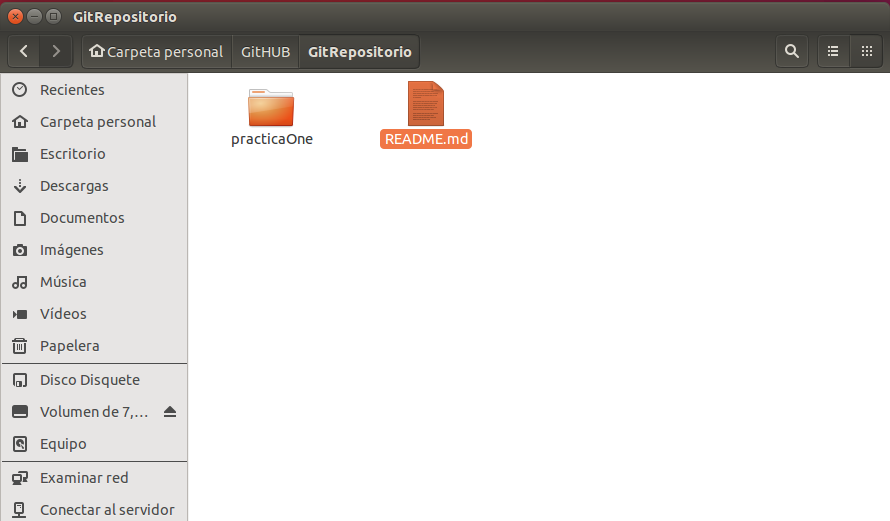
\includegraphics[width=8cm, height=5cm]{img/catorce}
%\textbf{Fig. 2 : Suscribirse a VPository }\\
\end{center}
\end{frame}



\begin{frame}
\frametitle{Desarrollo}

\setlength{\parskip}{03pt}
\begin{center}
\begin{itemize}
\justifying
\item{Accederemmos desde el terminal a la carpeta del repositorio y haremos un login con el nombre de usuario y el correo de nuestra cuenta github desde la terminal para subir el proyecto.}\end{itemize} 
\setlength{\parskip}{08pt}
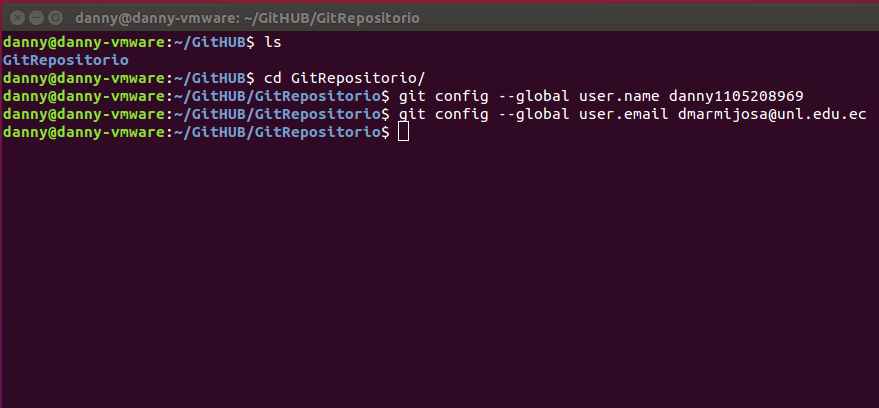
\includegraphics[width=8cm, height=5cm]{img/quince}
%\textbf{Fig. 2 : Suscribirse a VPository }\\
\end{center}
\end{frame}


\begin{frame}
\frametitle{Desarrollo}
\setlength{\parskip}{00pt}
Abrimos nuevamene el git gui colocando el codigo en la terminal \textbf{git gui} y haremos seleccionamos los archivos, colocamos un mensaje y le hacemos clic en commit para subir los archivos, si todo sale bien nos quedaria en blanco de nuevo. 
\begin{center}

\setlength{\parskip}{08pt}
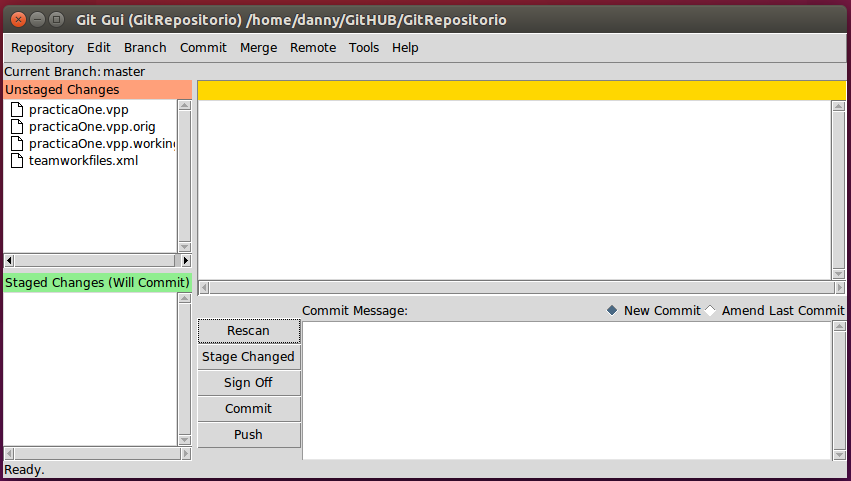
\includegraphics[width=5cm, height=3cm]{img/dieciseis} \hspace{0.5cm}
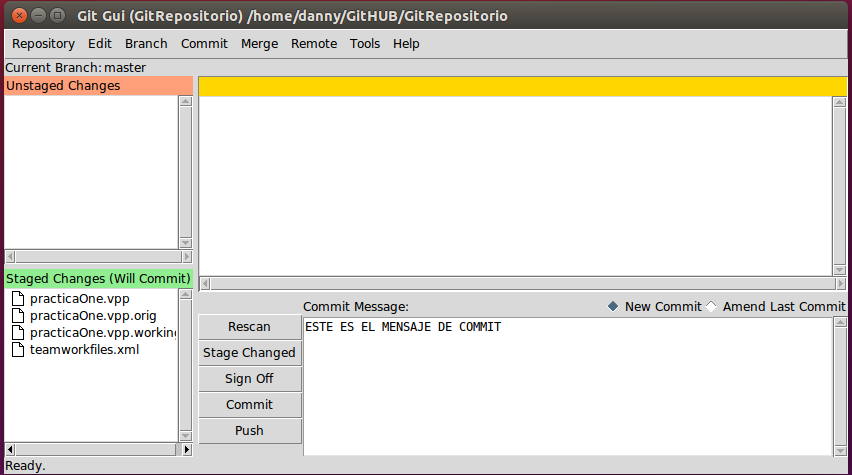
\includegraphics[width=4cm, height=3cm]{img/diecisiete}
%\textbf{Fig. 3 : Confirmación VPository }
\end{center}
\end{frame}


\begin{frame}
\frametitle{Desarrollo}
\setlength{\parskip}{03pt}
\begin{center}
\begin{itemize}
\justifying
\item{Para Asegurar que todo este bien para subir los archivos al repositorio, cerramos el git gui y abrimos una terminal, nos dirigimos al directorio de nuestro repositorio y colocamos la siguiente linea de comando \textbf{git pull origin master} y no debe darnos ningún error.}\end{itemize} 
\setlength{\parskip}{08pt}
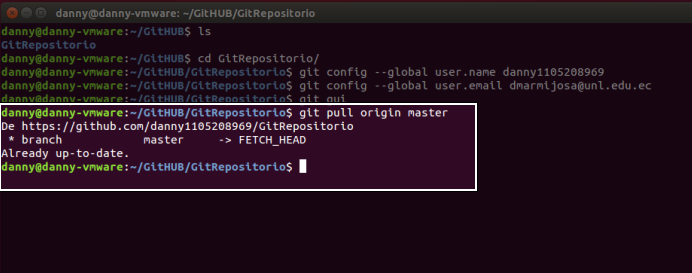
\includegraphics[width=10cm, height=5cm]{img/dieciocho}
%\textbf{Fig. 2 : Suscribirse a VPository }\\
\end{center}
\end{frame}


\begin{frame}
\frametitle{Desarrollo}
\setlength{\parskip}{03pt}
\begin{center}
\begin{itemize}
\justifying
\item{Confirmamos la subida con la siguiente linea de comando. \textbf{git push origin master}, luego ingresamos a \url{www.github.com} y ingresamos a nuestro repositorio con nuestro usuario y contraseña y verificamos que los datos hayan subid correctamente.}\end{itemize} 
\setlength{\parskip}{08pt}
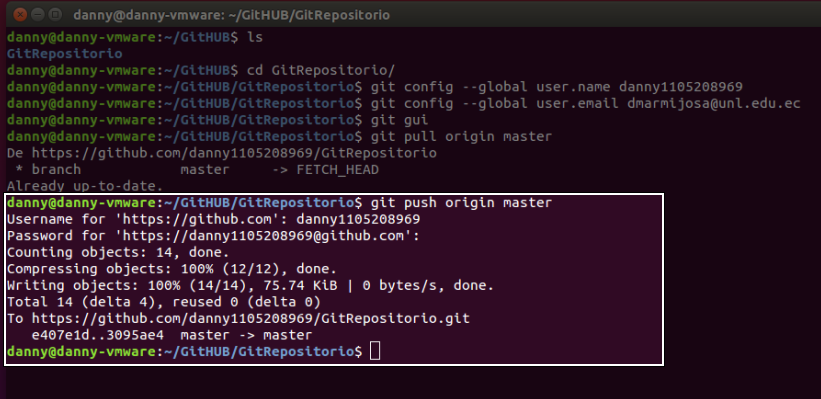
\includegraphics[width=10cm, height=5cm]{img/diecinueve}
%\textbf{Fig. 2 : Suscribirse a VPository }\\
\end{center}
\end{frame}



\begin{frame}
\frametitle{Desarrollo}
\setlength{\parskip}{03pt}
\begin{center}
\begin{itemize}
\justifying
\item{Revisamos en el repositorio de \url{www.github.com} y veremos que se ha subido correctamente nuestros archivos al repositorio y estan listos para ser compartidos.}
\end{itemize} 
\setlength{\parskip}{08pt}
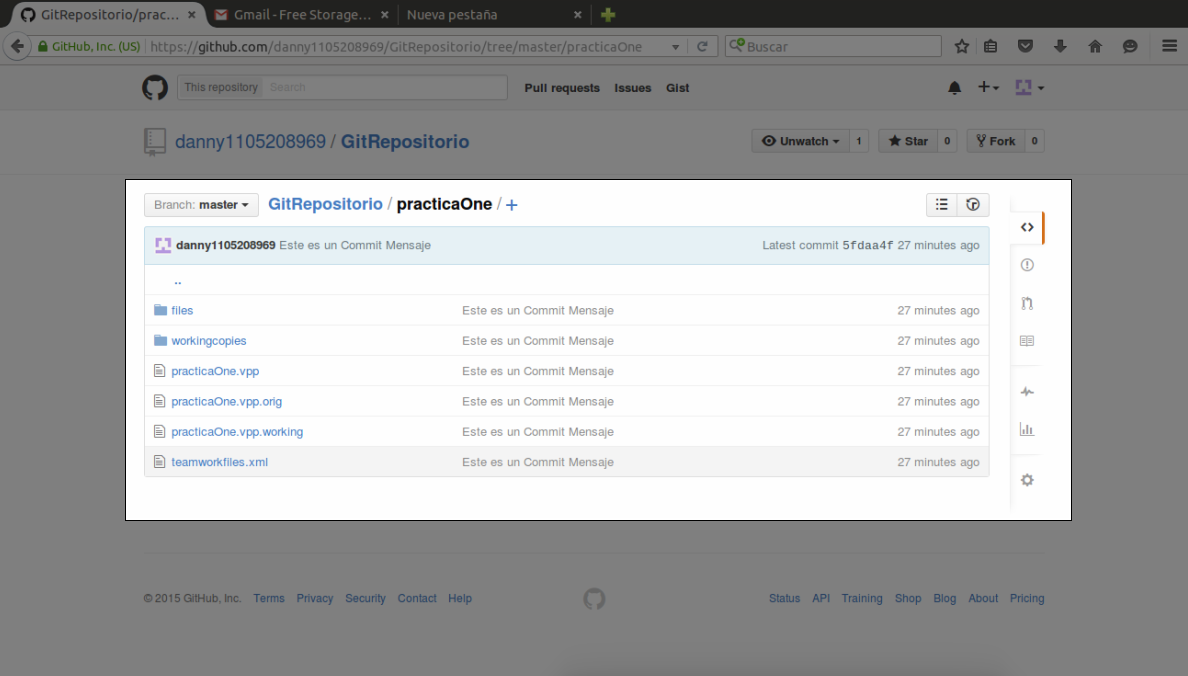
\includegraphics[width=10cm, height=5cm]{img/veinte}
%\textbf{Fig. 2 : Suscribirse a VPository }\\
\end{center}
\end{frame}


%/////////////////////////////////////
\subsubsection{EJEMPLO}
\begin{frame}
\frametitle{EJEMPLO}
\begin{enumerate}[1. ]
	\justifying
    \item Primeramente ingresamos a nuestro navegador e ingresamos a la dirección \url{http://www.github.com/}, luego de ello pulsamos en Sign In
\end{enumerate}
\begin{center}
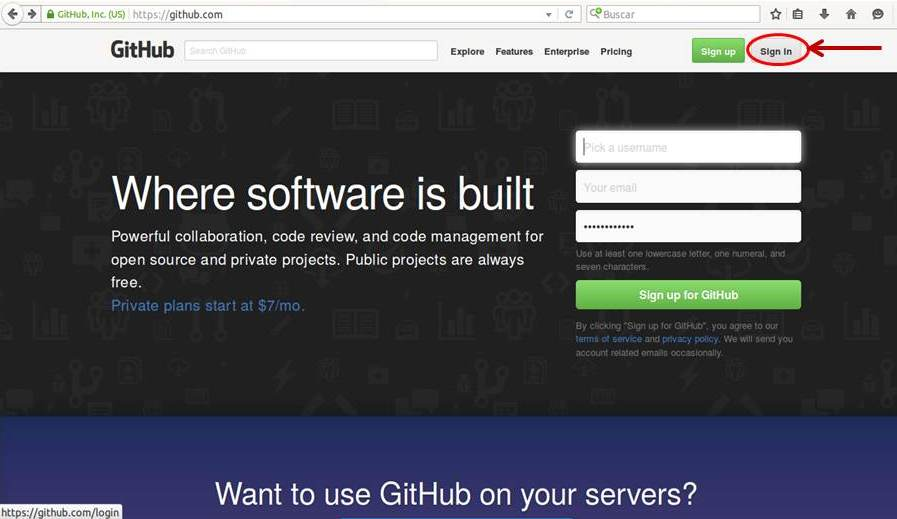
\includegraphics[width=9 cm]{img/b1}\
\textbf{Figura : Ingreso a GitHub}
\end{center}
\end{frame}

\begin{frame}
\frametitle{EJEMPLO}
\begin{enumerate}[2. ]
	\justifying
    \item Para ingresar debemos utilizar nuestro correo o nuestro username que ingresamos al momento de la configuración inicial, junto a nuestra password.
\end{enumerate}
\begin{center}
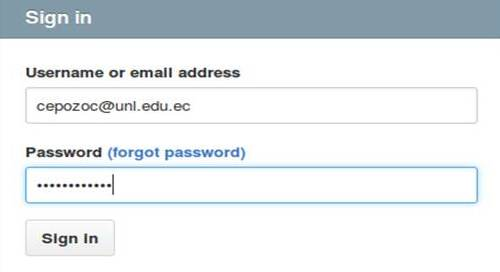
\includegraphics[width=9 cm]{img/b2}\\
\textbf{Figura : Ventana de Login de GitHub}
\end{center}
\end{frame}

\begin{frame}
\frametitle{EJEMPLO}
\begin{enumerate}[3. ]
	\justifying
    \item En la parte de la izquierda de nuestra cuenta GitHub, hay una sección en la que nos muestra nuestros repositorios que tengamos creados, podemos crear uno nuevo con New Repository.
\end{enumerate}
\begin{center}
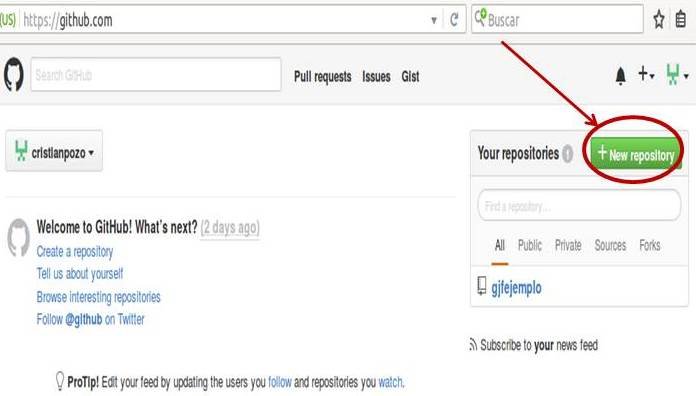
\includegraphics[width=6 cm]{img/b3}\\
\textbf{Figura : Área de Repositorios}
\end{center}
\end{frame}

\begin{frame}
\frametitle{EJEMPLO}
\begin{enumerate}[4. ]
	\justifying
    \item Escribimos el nombre del repositorio, y también seleccionamos Public, para que sea de acceso publico y seleccionamos Initialize this repository with a README.
\end{enumerate}
\begin{center}
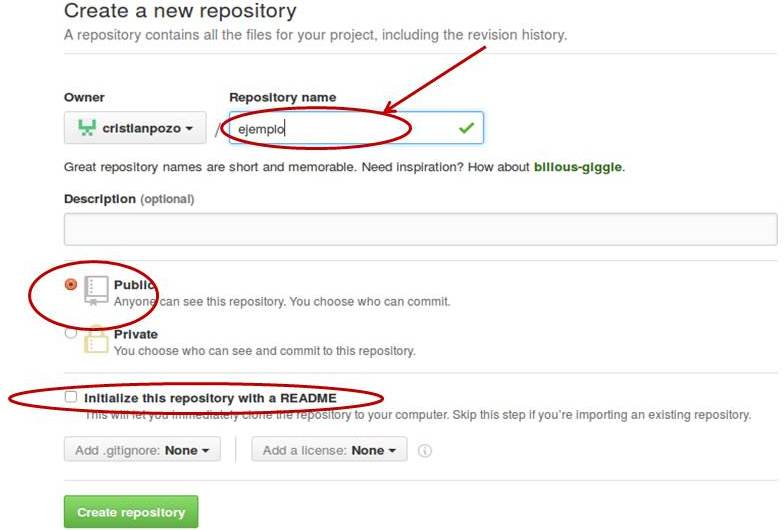
\includegraphics[width=7.5 cm]{img/b4}\\
\fontfamily{ppl}\fontsize{6}{1}\selectfont{\textbf{Figura : Ingreso a GitHub}}
\end{center}
\end{frame}

\begin{frame}
\frametitle{EJEMPLO}
\begin{enumerate}[5. ]
	\justifying
    \item Copiamos el URL del Repositorio el que queremos trabajar o compartirlo,luego de ello abrimos una terminal, nos dirigimos a la carpeta en la cual vamos a almacenar nuestro repositorio, para poder trabajar desde github.
\end{enumerate}
\begin{center}
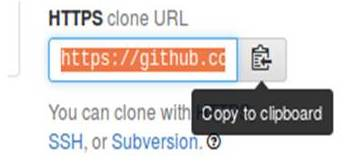
\includegraphics[width=3.5cm]{img/b5}\\

\includegraphics[width=7 cm]{img/b6}\\
\fontfamily{ppl}\fontsize{6}{1}\selectfont{\textbf{Figura : URL del Repositorio Git y la Consola de Ubuntu}}
\end{center}
\end{frame}

\begin{frame}
\frametitle{EJEMPLO}
\begin{enumerate}[6. ]
	\justifying
    \item Ingresamos a la carpeta en donde queremos clonar nuestro repositorio GitHub, luego de ello pegamos la dirección URL que copiamos  anteponiendo el comando git clone URLCopiada\\
\end{enumerate}
\begin{center}

\includegraphics[width=10cm]{img/b7}\\
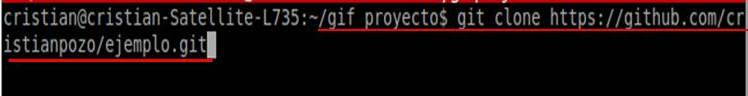
\includegraphics[width=10cm]{img/b8}\\
\fontfamily{ppl}\fontsize{6}{1}\selectfont{\textbf{Figura : URL del Repositorio Git y la Consola de Ubuntu}}
\end{center}
\end{frame}

\begin{frame}
\frametitle{EJEMPLO}
\begin{enumerate}[7. ]
	\justifying
    \item Luego de ello, como ya estamos dentro de la carpeta que clonamos nuestro repositorio, listamos nuestros repositorios con ls, y nos aseguramos que se haya clonado, si es así nos aparecerá un directorio con el mismo nombre del que clonamos.\\
\end{enumerate}
\begin{center}
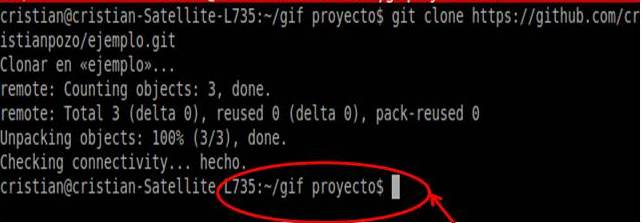
\includegraphics[width=7cm]{img/b9}\\
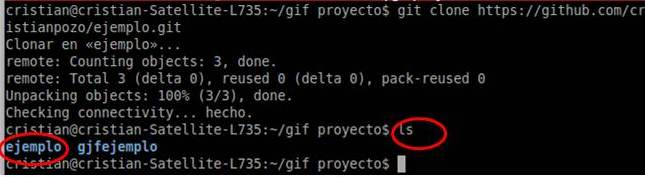
\includegraphics[width=7cm]{img/b10}\\
\fontfamily{ppl}\fontsize{6}{1}\selectfont{\textbf{Figura : Verificación de nuestro Repositorio GitHug Clonado}}
\end{center}
\end{frame}

\begin{frame}
\frametitle{EJEMPLO}
\begin{enumerate}[8. ]
	\justifying
    \item Luego ingresamos a Visual Paradingm, para constatar de que nuestro repositorio esté bien configurado, y que podamos trabajar. Para ello creamos un proyecto nuevo y luego hacemos un diagrama cualquiera, ya que en esta ocasión nos servirá simplemente como ejemplo.\\
\end{enumerate}
\begin{center}
\includegraphics[width=4cm]{img/b11}\\
\includegraphics[width=4.5cm]{img/b12}\\
\fontfamily{ppl}\fontsize{6}{1}\selectfont{\textbf{Figura : Ventana de Proyecto Nuevo en Visual Paradigm y Ejemplo de Caso de Uso.}}
\end{center}
\end{frame}

\begin{frame}
\frametitle{EJEMPLO}
\begin{enumerate}[9. ]
	\justifying
    \item Vamos a Save As, y nos dirigimos hacia el repositorio clonado Lo almacenamos, para luego de ello cargarlo a nuestro Repositorio GitHub\\
\end{enumerate}
\begin{center}
\includegraphics[width=7cm]{img/b13}\\
\fontfamily{ppl}\fontsize{6}{1}\selectfont{\textbf{Figura : Ventana de Guardar en Visual Paradigm}}
\end{center}
\end{frame}

\begin{frame}
\frametitle{EJEMPLO}
\begin{enumerate}[10. ]
	\justifying
    \item Nos dirigimos a nuestra consola, estando en la carpeta en donde tenemos nuestros repositorios clonados, luego de ello ingresamos al repositorio en el que guardamos nuestro proyecto .vpp que creamos, y escribimos el comando git gui, que es el que nos abrirá nuestra interfaz para guardar nuestro proyecto en la GitHub.\\
\end{enumerate}
\begin{center}
\includegraphics[width=7cm]{img/b14}\\
\fontfamily{ppl}\fontsize{6}{1}\selectfont{\textbf{Figura : Comando Para Abrir Nuestro Git Gráfico.}}
\end{center}
\end{frame}

\begin{frame}
\frametitle{EJEMPLO}
\begin{enumerate}[11. ]
	\justifying
    \item En nuestro entorno Git Gráfico, presionamos en Open Existing Repository para abrir nuestro repositorio, luego de ello seleccionamos el repositorio donde guardamos nuestro Proyecto de .vpp, luego presionamos OK.\\
\end{enumerate}
\begin{center}
\includegraphics[width=4.5cm]{img/b15}
\includegraphics[width=5cm]{img/b16}\\
\fontfamily{ppl}\fontsize{6}{1}\selectfont{\textbf{Figura : Comando Para Abrir Nuestro Git Gráfico.}}
\end{center}
\end{frame}

\begin{frame}
\frametitle{EJEMPLO}
\begin{enumerate}[12. ]
	\justifying
    \item Nos aparecerá nuestros archivos que se guardaron, luego de ello presionamos Scan, para indicar que los vamos a guardar en la GitHub, luego de esto presionamos Commit, para cargarlos a nuestros archivos.\\
\end{enumerate}
\begin{center}
\includegraphics[width=6.5cm]{img/b18}\\
\fontfamily{ppl}\fontsize{6}{1}\selectfont{\textbf{Figura : Comando Para Abrir Nuestro Git Gráfico.}}
\end{center}
\end{frame}

\begin{frame}
\frametitle{EJEMPLO}
\begin{enumerate}[13. ]
	\justifying
    \item Luego, nos dirigimos a la cansola que tenemos abierta, y le indicamos a github que vamos a subir cambios en nuestro repositorio clonado con el comando git pull origin master. Luego ingresamos el comando git push origin master para subir nuestros cambios, éste nos pedirá nuestro usuario GitHub y nuestro password, tendremos que ingresarlo.\\
\end{enumerate}
\begin{center}
\includegraphics[width=6 cm]{img/b20}\\
\includegraphics[width=6 cm]{img/b21}\\
\fontfamily{ppl}\fontsize{6}{1}\selectfont{\textbf{Figura : Comandos para subir nuestros archivos}}
\end{center}
\end{frame}

\begin{frame}
\frametitle{EJEMPLO}
\begin{enumerate}[14. ]
	\justifying
    \item Constatamos que en nuestro repositorio GitHub se hallan subido los cambios. Luego de esto vamos a agregar a un colaborador en nuestro proyecto, y para de esta manera poderlo trabajar con diferntes personas. Nos ubicamos en nuestro repositorio y presionamos en Settings.\\
\end{enumerate}
\begin{center}
\includegraphics[width=8 cm]{img/b23}\\
\fontfamily{ppl}\fontsize{6}{1}\selectfont{\textbf{Figura : Ingreso de nuevos Colaboradores.}}
\end{center}
\end{frame}

\begin{frame}
\frametitle{EJEMPLO}
\begin{enumerate}[15. ]
	\justifying
    \item Nos hubicamos en Collaborators, ahi nos da un espacio donde escribir al usuario con quien vamos a trabajar nuestro proyecto, ingresamos su id o su correo electrónico, luego presionamos Add Collaborators, y constatamos que en la parte superior se halla agregado.\\
\end{enumerate}
\begin{center}
\includegraphics[width=6 cm]{img/b25}\\
\fontfamily{ppl}\fontsize{6}{1}\selectfont{\textbf{Figura : Agregación de Colaboradores.}}
\end{center}
\end{frame}

\begin{frame}
\frametitle{EJEMPLO}
\begin{enumerate}[16. ]
	\justifying
    \item En la cuenta de nuestro colaborador debería aparecerle el repositorio al que se le agregó como colaborador. Antes de eso, le llega una notificación a su correo asociado a su cuenta GitHub. \\
\end{enumerate}
\begin{center}
\includegraphics[width=9 cm]{img/b26}\\
\fontfamily{ppl}\fontsize{6}{1}\selectfont{\textbf{Figura : Vista en Cuenta GitHub del Colaborador}}
\end{center}
\end{frame}

\begin{frame}
\frametitle{EJEMPLO}
\begin{enumerate}[17. ]
    \item  Aqui está la vista del Repositorio Compartido en la cuenta del Colaborador\\
\end{enumerate}
\begin{center}
\includegraphics[width=9 cm]{img/b27}\\
\fontfamily{ppl}\fontsize{6}{1}\selectfont{\textbf{Figura : Repositorio compartido}}
\end{center}
\end{frame}

\begin{frame}
\frametitle{EJEMPLO}
\begin{enumerate}[18. ]
	\justifying
    \item  El colaborador debe dirigirse a la carpeta donde él tiene sus repositorios clonados, y debe clonar también el repositorio compartido, copiando la URL como lo hizo el dueño del proyecto original, para poder trabajar de una manera local con el repositorio compartido.\\
\end{enumerate}
\begin{center}
\includegraphics[width=8cm]{img/b29}\\
\fontfamily{ppl}\fontsize{6}{1}\selectfont{\textbf{Figura : Repositorio compartido}}
\end{center}
\end{frame}

\begin{frame}
\frametitle{EJEMPLO}
\begin{enumerate}[19. ]
    \item Se clona el repositorio que se compartió, para poder trabajarlo localmente.\\
\end{enumerate}
\begin{center}
\includegraphics[width=8cm]{img/b30}\\
\fontfamily{ppl}\fontsize{6}{1}\selectfont{\textbf{Figura : Repositorio compartido}}
\end{center}
\end{frame}

\begin{frame}
\frametitle{EJEMPLO}
\begin{enumerate}[20. ]
	\justifying
    \item Para ver el proyecto compartido, se debe abrir Visual Paradigm, y se lo debe abrir con éste, ya que es de extensión .vpp, para trabajarlo aqui.\\
\end{enumerate}
\begin{center}
\includegraphics[width=7cm]{img/b31}\\
\fontfamily{ppl}\fontsize{6}{1}\selectfont{\textbf{Figura : Ventana de Proyectos en Visual Paradigm}}
\end{center}
\end{frame}

\begin{frame}
\frametitle{EJEMPLO}
\begin{enumerate}[21. ]
    \item El colaborador, hace una modificación, para comprobar que podemos trabajar con Visual Paradigm\\
\end{enumerate}
\begin{center}
\includegraphics[width=7cm]{img/b32}\\
\fontfamily{ppl}\fontsize{6}{1}\selectfont{\textbf{Figura : Modificación de Diagrama}}
\end{center}
\end{frame}

\begin{frame}
\frametitle{EJEMPLO}
\begin{enumerate}[22. ]
    \item El colaborador,debe seguir el mismo procedimiento que siguió el usuario que creó le proyecto, para cargar la modificación realizada.\\
\end{enumerate}
\begin{center}
\includegraphics[width=7cm]{img/b33}\\
\fontfamily{ppl}\fontsize{6}{1}\selectfont{\textbf{Figura : Almacenamiento de la modificación en GitHub}}
\end{center}
\end{frame}

\begin{frame}
\frametitle{EJEMPLO}
\begin{enumerate}[23. ]
	\justifying
    \item En la cuenta del Autor del Proyecto, llega una notifiación del Proyecto, en la que le informa que existe una modificación por parte del colaborador a quien lo hizo formar parte del proyecto. Deberrá Aprobarlo.\\
\end{enumerate}
\begin{center}
\includegraphics[width=7cm]{img/b35}\\
\fontfamily{ppl}\fontsize{6}{1}\selectfont{\textbf{Figura : Almacenamiento de la modificación en GitHub}}
\end{center}
\end{frame}

\begin{frame}
\frametitle{EJEMPLO}
\begin{enumerate}[24. ]
	\justifying
    \item Luego de haberlo aprobado, se diría que el proyecto tuvo una modificacion por parte de un colaborador, o que hay una nueva versión del proyexto. Como vemos, se ven las modificaciones con la fecha, y con la hora de modificación.\\
\end{enumerate}
\begin{center}
\includegraphics[width=7cm]{img/b36}\\
\fontfamily{ppl}\fontsize{6}{1}\selectfont{\textbf{Figura : Ventana de Proyecto modificado}}
\end{center}
\end{frame}

\begin{frame}
\frametitle{EJEMPLO}
\begin{enumerate}[24. ]
	\justifying
    \item Vemos que la modificación se concretó, para ello el autor del proyecto sigue el mismo procedimiento que lo hizo el colaborador para revisar el proyecto, esta vez lo abrirá y revisará que se ha modificado.\\
\end{enumerate}
\begin{center}
\includegraphics[width=7cm]{img/b37}\\
\fontfamily{ppl}\fontsize{6}{1}\selectfont{\textbf{Figura : Verificación de Cambios en el proyecto}}
\end{center}
\end{frame}

\subsection{Conclusiones}
\begin{frame}
\frametitle{Conclusiones}
Luego de haber realizado el presente trabajo, hemos llegado a las siguientes conclusiones:
\begin{itemize}
\justifying
\item Las herramientas de almacenamiento en la nube, nos permiten alojar de una mejor manera la información, y así poder, además de acceder a ella, trabajar nuestros proyectos, indistintamente de la ubicación geográfica donde se encuentren.
\justifying
\item Las plataformas de Desarrollo Colaborativo, nos brindan facilidad y flexibilidad para el desarrollo de software, ya que además de almacenar y compartir proyectos, nos brindan sistemas de control de versiones, las mismas que nos permiten revisar modificaciones que se lleven a cabo en nuestros proyectos para poderlas aprobar o rechazar.
\end{itemize}
\end{frame}

\subsection{Bibliografía}
\begin{frame}
\frametitle{Bibliografia}
	\begin{enumerate}
		\item Paradigm, V. (2013). Visual paradigm for uml. Visual Paradigm for UML-UML tool for software application development.
		\item \url{https://git-scm.com}
		\item \url{https://developer.github.com/v3/}
		\item J. Soto, Mi Primer Libro.  Concepción, Chile: McGraw-Hill, 2013.
		\item J. Soto, Mi Primer Libro.  Concepción, Chile: McGraw-Hill, 2013.
		
	\end{enumerate}
\end{frame}

\subsection{Licencia}
\begin{frame}
\frametitle{Licencia}
\begin{center}
\href{http://www.google.com}{\includegraphics[scale=.8]{cc}}
\end{center}
\end{frame}

\MuchasGraciasFrame

\end{document}